\documentclass{article}
\usepackage{../../Self_Style}

\title{Phys 20AL Week 7: Driven Harmonic Oscillator 2}
\author{Zih-Yu Hsieh}
\date{\today}

\begin{document}
\maketitle

\tableofcontents

\newpage

\section{Aim of the Report}
This aims to use a more controlled version of the driven harmonic oscillator, to observe the effect of resonance on the amplitude and phase difference when given a driven harmonic oscillator, and calculate the given damping constant $\gamma$.

\hfil

For the provided experiment, instead of fixing the length of the driving pendulum (which has mass $500$ g), it fixes the the natural frequency of the pendulum that's being driven (so $w_0$ is fixed), while varying the length of the driving pendulum (which varies the driving frequency $w$). Which, the data analysis splits into multiple steps:
\begin{enumerate}
    \item Establish the value of $\omega_0$.
    \item Establish the initial driven frequency $w$, together with the initial length $L_0$ of the large driving pendulum.
    \item Use the above $L_0$ to predict the driven frequency when changing to different lengths (including $+1,1.5,2,2.25,2.5,2.75,3,3.25,3.5,4,4.5,5.55,6.5$ in.).
    \item Calculate the actual driven frequency under different lengths, and make comparison to the predicted data.
    \item Gather the driven pendulum's amplitude and phase difference compared to the large driving pendulum.
\end{enumerate}
Which, we'll gather a total of $4$ peaks in each video (for both the large driving pendulum, and the small driven pendulum) to gather a total of $3$ periods for calculation with phase difference, and also use the first three peaks as the reference for amplitude.

\newpage

\section{Natural Frequency $w_0$:}
Under the video, the three compared trials each has period $T = 2.440, 2.380, 2.440$ s, which provides an average period $T_\text{ave} = 2.420$ s, and standard deviation $\delta_T =0.035$ s.

As a result, since natural frequency $w = \frac{2\pi}{T}$ with $T$ being the period, then the calculated natural frequency is $w_0 = \frac{2\pi}{T_\text{ave}} \approx 2.596$ rad/s; and, since $\frac{\partial w}{\partial T} = -\frac{2\pi}{T^2}$, the propogation of uncertainty is given by $\delta w_0 = \left|\frac{\partial w_0}{\partial T}\delta T\right| = \frac{2\pi}{2.42^2}0.035 \approx 0.038$ rad/s.

One can see that in comparison to the $w_0$ calculated, $\delta w_0$ is relatively small, hence there is a high confidence one can say this represents the actual natural frequency $w_0$.

\hfil

\section{Initial Length $L_0$, and Initial Driving Frequency $w$:}
From the video of the large driving pendulum (with initial length), the three collected period are given by $T=2.300,2.370,2.360$ s, which provides an average period $T_\text{ave} \approx 2.343$ s, and standard deviation $\delta T\approx 0.038$ s.

Which, with the frequency $w = \frac{2\pi}{T}$ (where $T$ is the period), the driven frequency is given by $w = \frac{2\pi}{T} = \frac{2\pi}{2.343} \approx 2.682$ rad/s; and, the propogation of uncertainty is $\delta w=\left|\frac{\partial w}{\partial T}\delta t\right| = \frac{2\pi}{2.343^2}0.038\approx 0.043$ rad/s.

So, one can see the uncertainty $\delta w$ is relatively small in comparison to the calculated initial driven frequency $w$, showing there is a high confidence this $w$ value represents the initial driven frequency.

\hfil

On the other hand, with period of the pendulum $T = 2\pi\sqrt{\frac{l}{g}}$ (where $l$ is the length of the pendulum), then $l = \frac{gT^2}{4\pi^2}$, so with average driving period $T_\text{ave} \approx 2.343$ s, the calculated initial length $L_0 = \frac{gT^2}{4\pi^2} \approx 1.364$ m. Also, since $\frac{\partial l}{\partial T} = \frac{gT}{2\pi^2}$, then the propogation of uncertainty is given by $\delta L_0 = \left|\frac{\partial l}{\partial T}\delta T\right| = \frac{g T_\text{ave}}{2\pi^2}0.038 \approx \frac{9.807 \cdot 2.343}{2\pi^2}0.038 \approx 0.044$ m.

One can see also that in comparison to the calculated initial length $L_0$, the uncertainty $\delta L_0$ is relatively small, so there is also a high confidence one can say that the $L_0$ represents the initial length of the large driving pendulum.

\hfil

\section{Prediction of Driven Frequency}
Given the calculated initial length $L_0 \approx 1.364$ m, then with the formula of frequency $w =\sqrt{\frac{g}{l}}$, each of the added length provides the following:
\begin{table}[h!]
\centering
\begin{tabular}{c||cccccccccccccc}
\hline
$+l$ (in.) &
0.000 & 1.000 & 1.500 & 2.000 & 2.250 & 2.500 & 2.750 &
3.000 & 3.250 & 3.500 & 4.000 & 4.500 & 5.500 & 6.500 \\
\hline
$L_0+l$ (m) &
1.364 & 1.389 & 1.402 & 1.415 & 1.421 & 1.428 & 1.434 &
1.440 & 1.447 & 1.453 & 1.466 & 1.478 & 1.504 & 1.529 \\
\hline
$\omega$ (rad/s) &
2.681 & 2.657 & 2.645 & 2.633 & 2.627 & 2.621 & 2.615 &
2.609 & 2.604 & 2.598 & 2.587 & 2.576 & 2.554 & 2.532 \\
\hline
\end{tabular}
\caption{Table of Total Length and Predicted Angular Frequency}
\label{tab:predict_w}
\end{table}

\hfil

\section{Collected Driven Frequency, and Comparison:}
First, using the given videos, together with the frequency formula $w=\frac{2\pi}{T}$ (where $T$ is the given period), and the propogation of uncertainty $\delta w = \left|\frac{\partial w}{\partial T}\delta T\right| = \frac{2\pi}{T^2}\delta T$, the collected 3 periods for each pendulum length, average period $T_\text{ave}$, RMSD of period $\delta T$ have provided the following table:
\begin{table}[h!]
\centering
\scriptsize
\begin{tabular}{c||ccc||c|c||c|c}
\hline
\diagbox[width=3cm,height=1cm]{\textbf{$L_0+l$ (m)}}{\textbf{Trial}} &
\textbf{1} & \textbf{2} & \textbf{3} &
\textbf{$T_\text{ave}$ (s)} & \textbf{$\delta T$ (s)} &
\textbf{$\omega$ (rad/s)} & \textbf{$\delta \omega$ (rad/s)} \\
\hline
\hline
1.364 & 2.300 & 2.370 & 2.360 & 2.343 & 0.038 & 2.681 & 0.043 \\
1.389 & 2.330 & 2.380 & 2.360 & 2.357 & 0.025 & 2.666 & 0.028 \\
1.402 & 2.340 & 2.370 & 2.410 & 2.373 & 0.035 & 2.647 & 0.039 \\
1.415 & 2.370 & 2.400 & 2.400 & 2.390 & 0.017 & 2.629 & 0.019 \\
1.421 & 2.440 & 2.340 & 2.370 & 2.383 & 0.051 & 2.636 & 0.057 \\
1.428 & 2.400 & 2.420 & 2.400 & 2.407 & 0.012 & 2.611 & 0.013 \\
1.434 & 2.420 & 2.400 & 2.430 & 2.417 & 0.015 & 2.600 & 0.016 \\
1.440 & 2.420 & 2.380 & 2.440 & 2.413 & 0.031 & 2.604 & 0.033 \\
1.447 & 2.440 & 2.420 & 2.410 & 2.423 & 0.015 & 2.593 & 0.016 \\
1.453 & 2.400 & 2.410 & 2.430 & 2.413 & 0.015 & 2.604 & 0.016 \\
1.466 & 2.400 & 2.450 & 2.400 & 2.417 & 0.029 & 2.600 & 0.031 \\
1.478 & 2.420 & 2.470 & 2.420 & 2.437 & 0.029 & 2.579 & 0.031 \\
1.504 & 2.420 & 2.430 & 2.490 & 2.447 & 0.038 & 2.568 & 0.040 \\
1.529 & 2.460 & 2.480 & 2.440 & 2.460 & 0.020 & 2.554 & 0.021 \\
\hline
\end{tabular}
\caption{Table of measured Driven Period $T$, and calculated Driven Frequency $w$}
\label{tab:calc_driven_w}
\end{table}

\hfil

Which, the comparison between the prediction is as follow (together with provided percent error):
\begin{table}[h!]
\centering
\begin{tabular}{c|c|c|c}
\hline
\textbf{$L_0+l$ (m)} &
\textbf{Predicted $\omega$ (rad/s)} &
\textbf{Calculated $\omega$ (rad/s)} &
\textbf{Percent Error (\%)} \\
\hline
\hline
1.364 & 2.681 & 2.681 & 0.000 \\
1.389 & 2.657 & 2.666 & 0.354 \\
1.402 & 2.645 & 2.647 & 0.105 \\
1.415 & 2.633 & 2.629 & 0.144 \\
1.421 & 2.627 & 2.636 & 0.359 \\
1.428 & 2.621 & 2.611 & 0.393 \\
1.434 & 2.615 & 2.600 & 0.586 \\
1.440 & 2.609 & 2.604 & 0.226 \\
1.447 & 2.604 & 2.593 & 0.420 \\
1.453 & 2.598 & 2.604 & 0.213 \\
1.466 & 2.587 & 2.600 & 0.509 \\
1.478 & 2.576 & 2.579 & 0.118 \\
1.504 & 2.554 & 2.568 & 0.558 \\
1.529 & 2.532 & 2.554 & 0.850 \\
\hline
\end{tabular}
\caption{Predicted vs. Calculated Driven Frequency of the Data}
\label{tab:compare_w}
\end{table}

One can see that the predicted and the calculated driven frequency are in fact having a small error (which can be seen by the fact that the percent errors are all bounded below $0.9\%$), showing the experimental data in fact highly agree with the predicted values.

\newpage

\section{Amplitude}
Using the videos, each given length of the large driving pendulum corresponded to 3 trials of amplitude (unit: m). Which, the average amplitude $x_\text{max, ave}$, together with the RMSD value $\delta x_\text{max}$ is given as follow:
\begin{table}[h!]
\centering
\scriptsize
\begin{tabular}{c||ccc||c|c}
\hline
\diagbox[width=3cm,height=1cm]{\textbf{$L_0+l$ (m)}}{\textbf{Trial}} &
\textbf{1} & \textbf{2} & \textbf{3} &
\textbf{$x_\text{max, ave}$ (m)} & \textbf{$\delta x_\text{max}$ (m)} \\
\hline
\hline
1.364 & 0.055 & 0.055 & 0.055 & 0.055 & 0.000 \\
1.389 & 0.078 & 0.078 & 0.075 & 0.077 & 0.001 \\
1.402 & 0.078 & 0.080 & 0.080 & 0.079 & 0.001 \\
1.415 & 0.080 & 0.078 & 0.080 & 0.079 & 0.001 \\
1.421 & 0.078 & 0.080 & 0.083 & 0.080 & 0.003 \\
1.428 & 0.080 & 0.080 & 0.083 & 0.081 & 0.001 \\
1.434 & 0.088 & 0.090 & 0.093 & 0.090 & 0.003 \\
1.440 & 0.093 & 0.095 & 0.098 & 0.095 & 0.003 \\
1.447 & 0.093 & 0.095 & 0.098 & 0.095 & 0.003 \\
1.453 & 0.093 & 0.093 & 0.095 & 0.093 & 0.001 \\
1.466 & 0.095 & 0.098 & 0.100 & 0.098 & 0.003 \\
1.478 & 0.093 & 0.093 & 0.095 & 0.093 & 0.001 \\
1.504 & 0.078 & 0.080 & 0.080 & 0.079 & 0.001 \\
1.529 & 0.065 & 0.063 & 0.060 & 0.063 & 0.003 \\
\hline
\end{tabular}
\caption{Measured Amplitude of each Length}
\label{tab:meas_amp}
\end{table}

Which, they generate the following graph and fit line with respect to the driven frequency:
\begin{figure}[h!]
    \centering
    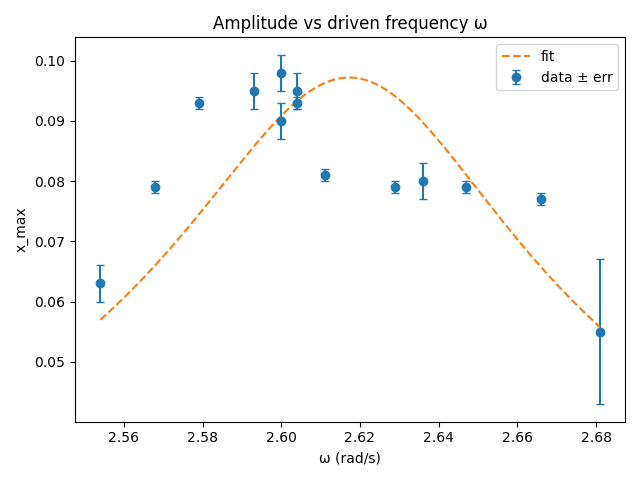
\includegraphics[width=130mm]{Amplitude w7.png}
\end{figure}

However, in comparison to the natural frequency $w_0 \approx 2.593$ rad/s, here one can see the maximum is learning more toward $w=2.62$ rad/s, instead of on the natural frequency (when the resonance actually happens). Hence, the line of best fit is not having a high validity of representing the predicted model here.

\newpage

\section{Phase}
Again, using the videos, each given length of the large driving pendulum corresponded to 3 trials of phase difference $\Delta t$ (unit: s). Which, the average phase difference $\Delta t_\text{ave}$, the RMSD value $\delta t$ can be calculated.

On top of that, since the phase difference $\delta := w\Delta t$ (where $w$ is the driven frequency), so using propogation of uncertainty, we have the uncertainty of phase difference $\delta_\text{err} = \sqrt{(\frac{\partial \delta}{\partial w}\delta w)^2+(\frac{\partial \delta}{\partial (\Delta t)}\delta t)^2} = \sqrt{(\Delta t\cdot \delta w)^2 + (w \cdot \delta t)^2}$. Then, the calculated values form the following table ($w,\delta w$ are in \textbf{Table \ref{tab:calc_driven_w}}):
\begin{table}[h!]
\centering
\scriptsize
\begin{tabular}{c||ccc||cc||cc}
\hline
\diagbox[width=3cm,height=1cm]{\textbf{$L_0+l$ (m)}}{\textbf{Trial}} &
\textbf{1} & \textbf{2} & \textbf{3} &
\textbf{$\Delta t_\text{ave}$ (s)} & \textbf{$\delta t$} &
\textbf{$\delta$} & \textbf{$\delta_\text{err}$} \\
\hline
\hline
1.364 & 0.940 & 1.020 & 1.010 & 0.990 & 0.044 & 0.044 & 0.000 \\
1.389 & 0.960 & 0.940 & 0.980 & 0.960 & 0.020 & 0.019 & 0.000 \\
1.402 & 0.740 & 0.790 & 0.780 & 0.770 & 0.026 & 0.021 & 0.000 \\
1.415 & 0.630 & 0.680 & 0.670 & 0.660 & 0.026 & 0.018 & 0.000 \\
1.421 & 0.660 & 0.610 & 0.640 & 0.637 & 0.025 & 0.015 & 0.000 \\
1.428 & 0.630 & 0.670 & 0.610 & 0.637 & 0.031 & 0.020 & 0.000 \\
1.434 & 0.570 & 0.570 & 0.550 & 0.563 & 0.012 & 0.007 & 0.000 \\
1.440 & 0.470 & 0.440 & 0.490 & 0.467 & 0.025 & 0.011 & 0.000 \\
1.447 & 0.440 & 0.390 & 0.420 & 0.417 & 0.025 & 0.010 & 0.000 \\
1.453 & 0.430 & 0.450 & 0.420 & 0.433 & 0.015 & 0.007 & 0.000 \\
1.466 & 0.300 & 0.280 & 0.270 & 0.283 & 0.015 & 0.004 & 0.000 \\
1.478 & 0.220 & 0.260 & 0.210 & 0.230 & 0.026 & 0.007 & 0.000 \\
1.504 & 0.130 & 0.170 & 0.150 & 0.150 & 0.020 & 0.003 & 0.000 \\
1.529 & 0.000 & 0.010 & 0.010 & 0.007 & 0.006 & 0.000 & 0.000 \\
\hline
\end{tabular}
\caption{Table of Phase Difference $\delta$ of each Length of Large Driving Pendulum}
\label{tab:phase}
\end{table}

Which, it generates the following graph:
\begin{figure}[h!]
    \centering
    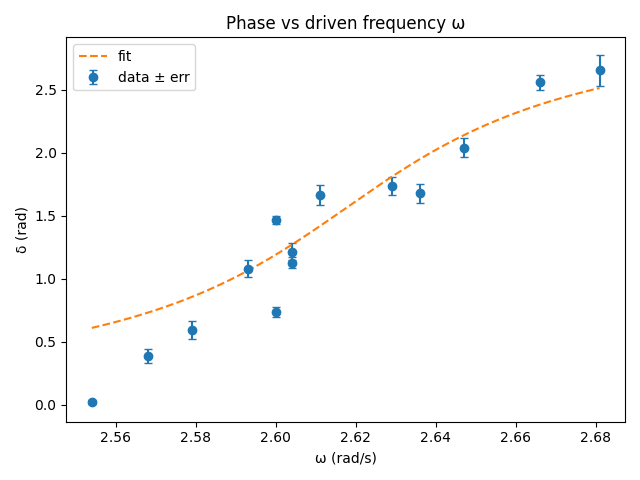
\includegraphics[width=130mm]{Phase w7.png}
\end{figure}

Similar to amplitude, the phase difference of $\frac{\pi}{2}\approx 1.57$ is on $w\approx2.61$ rad/s, instead of the natural frequency $w_0\approx 2.596$ rad/s, so the data still doesn't have a high validity of representing the model prediction in this case either. However, within the data used for interpolation, it's within the range $[0,\pi]$, showing that the calculated data is at least balid as a phase difference.

\hfil

\section{Calculated Coefficients and Conclusion}
Using the program to find the best fit line, if using the following two equations:
\begin{align}
    x_\text{max} = \frac{\alpha}{\sqrt{(w_0^2-w^2)^2+(2\gamma w)^2}},\quad \delta = \arctan\left(\frac{2\gamma w}{w_0^2-w^2}\right)
\end{align}
Then, the program returns the values $\alpha\approx 0.0226$, and $\gamma\approx 0.0448$ kg/s.

\hfil

In this report, one can see during the start when extracting both the length and driven frequency (caused by the large pendulum), the data has small uncertainty values, which the average has relatively high validity of representing what has happened in the experiemnt (or the videos provided). 

However, when plotting the graphs about the relations between driven frequency $w$, amplitude $x_\text{max}$, and phase difference $\delta$, one can see the data isn't really fitting with the prediction: For instance, the maximum of amplitude doesn't occure near $w\approx w_0$, but rather an explicitly higher value than $w_0$ (based on the best fit curve), similarly $\delta=\frac{\pi}{2}$ (which is where the max amplitude supposedly occurs based on formula prediction) also occurs at an explicitly higher value than $w_0$. 

Hence, in this experiment the formula prediction isn't fitting with the experimental result, showing it doesn't have a high validity of representing this experiment specifically.

\end{document}